% ============================================================================
% Lecture 22 (B21): Deep Surrogate Models
% Deep Learning for Solving and Estimating Dynamic Models in Economics and Finance
% Course author: Simon Scheidegger
% ============================================================================

\documentclass[aspectratio=169,11pt]{beamer}

% ---------- Theme and colors ----------
\usecolortheme{dove}
\setbeamertemplate{navigation symbols}{}
\setbeamertemplate{footline}{%
  \hfill\usebeamerfont{page number in head/foot}%
  \usebeamercolor[fg]{normal text}%
  \insertframenumber\,/\,\inserttotalframenumber\kern1em\vskip4pt}
\setbeamerfont{frametitle}{size=\huge}

% ---------- Packages ----------
\usepackage[utf8]{inputenc}
\usepackage[T1]{fontenc}
\usepackage{amsmath,amssymb,amsfonts}
\usepackage{bm}
\usepackage{graphicx}
\usepackage{tikz}
\usetikzlibrary{shapes,arrows.meta,positioning,calc,fit,backgrounds,patterns,decorations.pathreplacing}
\usepackage{pgfplots}
\pgfplotsset{compat=1.18}
\usepackage{booktabs}
\usepackage{hyperref}
\usepackage{multicol}
\usepackage{xcolor}
\usepackage{algorithm}
\usepackage{algorithmic}
\usepackage{listings}
\usepackage{pifont}

% ---------- Listings style for Python ----------
\lstset{
    language=Python,
    basicstyle=\small\ttfamily,
    keywordstyle=\color{uzhblue}\bfseries,
    commentstyle=\color{uzhgreydark}\itshape,
    stringstyle=\color{darkgreen},
    showstringspaces=false,
    breaklines=true,
    frame=none,
    xleftmargin=0pt,
    aboveskip=4pt,
    belowskip=4pt,
    escapeinside={(*@}{@*)},
}

% ---------- Custom colors ----------
\definecolor{uzhblue}{rgb}{0,0,0.5}
\definecolor{uzhgreylight}{RGB}{236,238,241}
\definecolor{uzhgreydark}{RGB}{81,86,94}
\definecolor{harvardcrimson}{RGB}{153,0,0}
\definecolor{unil@blue}{RGB}{0,140,204}
\definecolor{unil@black}{RGB}{35,31,32}
\definecolor{darkgreen}{RGB}{0,100,0}
\definecolor{darkred}{RGB}{139,0,0}
\definecolor{softblue}{RGB}{70,130,180}
\definecolor{softorange}{RGB}{230,159,0}
\definecolor{softgreen}{RGB}{0,158,115}

% ---------- Set beamer colors ----------
\setbeamercolor{frametitle}{bg=uzhgreylight, fg=uzhblue}
\setbeamercolor{title}{fg=uzhblue}
\setbeamercolor{structure}{fg=uzhblue}
\setbeamercolor{block title}{bg=unil@blue, fg=white}
\setbeamercolor{block body}{bg=uzhgreylight}
\setbeamercolor{block title alerted}{bg=darkred,fg=white}
\setbeamercolor{block body alerted}{bg=red!5}
\setbeamercolor{block title example}{bg=darkgreen,fg=white}
\setbeamercolor{block body example}{bg=green!5}
\setbeamercolor{item}{fg=unil@black}
\setbeamercolor{normal text}{fg=unil@black}

% ---------- Emphasis and hyperlinks ----------
\newcommand{\emphc}[1]{\textcolor{harvardcrimson}{#1}}
\hypersetup{colorlinks,linkcolor=harvardcrimson,urlcolor=harvardcrimson}

% ---------- Math commands ----------
\newcommand{\x}{\bm{x}}
\newcommand{\w}{\bm{w}}
\newcommand{\bb}{\bm{b}}
\newcommand{\z}{\bm{z}}
\newcommand{\W}{\bm{W}}
\newcommand{\X}{\bm{X}}
\renewcommand{\a}{\bm{a}}
\newcommand{\R}{\mathbb{R}}
\newcommand{\E}[1]{\mathbb{E}\!\left[#1\right]}
\DeclareMathOperator*{\argmin}{arg\,min}
\DeclareMathOperator*{\argmax}{arg\,max}

% ---------- Title ----------
\title[Lecture 24 (B23)]{Lecture 24 (B23): Bayesian Active Learning}
\subtitle{Where to sample, BAL algorithm, BAL in economics, BAL + GPs for surrogates}
\author{Simon Scheidegger}
\institute{HEC, University of Lausanne}
\date{}
\begin{document}

% Custom command used in some "Finger Exercise" frame titles.
\providecommand{\exercisepause}{%
  \tikz[baseline=(X.base)]{\node[fill=darkgreen!80!black, text=white,
  rounded corners=2pt, inner sep=3pt, font=\scriptsize\bfseries](X){PAUSE};}}

{\setbeamercolor{background canvas}{bg=uzhgreylight}
\begin{frame}
\titlepage
\end{frame}
}

\section{Bayesian Active Learning}

% --- Slide 33: Motivation ---
\begin{frame}{Motivation: Where to Sample?}
\begin{columns}[T]
\begin{column}{0.48\textwidth}
\textbf{Uniform sampling:}
\begin{itemize}
  \item Places points evenly across the domain
  \item Wastes evaluations in smooth regions
  \item Cannot adapt to function complexity
\end{itemize}
\end{column}
\begin{column}{0.48\textwidth}
\textbf{Adaptive / active sampling:}
\begin{itemize}
  \item Concentrates points where the function is \emphc{hard to approximate}
  \item Uses the model's \emphc{uncertainty} to guide selection
  \item Fewer evaluations for the same accuracy
\end{itemize}
\end{column}
\end{columns}

\vspace{0.5cm}
\begin{alertblock}{Key question}
Given a budget of $N$ model evaluations, which input points $\{x_1, \dots, x_N\}$ minimize the overall approximation error?
\end{alertblock}
\end{frame}

% --- Slide 34: BAL — The Idea ---
\begin{frame}{Bayesian Active Learning: The Idea}
\textbf{Use the GP posterior variance to guide sampling.}

\vspace{0.2cm}
\begin{block}{Acquisition / score function}
\vspace{-4pt}
\[
U(\x) = w_{\mathrm{exp}} \cdot \mu(\x) + \frac{w_{\mathrm{var}}}{2}\log\sigma^2(\x)
\]
\vspace{-8pt}
\begin{itemize}\setlength{\itemsep}{1pt}
  \item $\mu(\x)$: posterior mean (\emphc{exploitation} --- sample where function is large)
  \item $\sigma^2(\x)$: posterior variance (\emphc{exploration} --- sample where uncertainty is high)
  \item $w_{\mathrm{exp}}, w_{\mathrm{var}} \geq 0$: trade-off weights (distinct from the AR(1) coefficient $\rho$ and the discount factor $\beta$ used elsewhere).
\end{itemize}
\end{block}

\vspace{0.2cm}
\textbf{Pure exploration} ($w_{\mathrm{exp}} = 0$): maximize $\sigma^2(\x)$, i.e., uncertainty sampling.\\[3pt]
\textbf{Mixed} ($w_{\mathrm{exp}} > 0, w_{\mathrm{var}} > 0$): balance exploration and exploitation.\\[3pt]
{\small For surrogate building, pure exploration (max variance) is often sufficient.}
\end{frame}

% --- Slide 35: BAL Algorithm ---
\begin{frame}{BAL Algorithm}
\begin{algorithm}[H]
\caption{Bayesian Active Learning for Surrogates}
\begin{algorithmic}[1]
\REQUIRE Initial design $\mathcal{D}_0 = \{(\x_i, y_i)\}_{i=1}^{n_0}$, budget $N$, candidate set $\mathcal{C}$
\STATE Fit GP on $\mathcal{D}_0$: compute posterior mean $\mu(\cdot)$ and variance $\sigma^2(\cdot)$
\FOR{$t = 1, \dots, N - n_0$}
    \STATE Compute score $U(\x) = w_{\mathrm{exp}}\,\mu(\x) + \frac{w_{\mathrm{var}}}{2}\log\sigma^2(\x)$ for all $\x \in \mathcal{C}$
    \STATE Select $\x_{\text{new}} = \argmax_{\x \in \mathcal{C}} U(\x)$
    \STATE Query the expensive model: $y_{\text{new}} = f(\x_{\text{new}})$
    \STATE Update: $\mathcal{D}_t \leftarrow \mathcal{D}_{t-1} \cup \{(\x_{\text{new}}, y_{\text{new}})\}$
    \STATE Refit GP on $\mathcal{D}_t$
\ENDFOR
\RETURN Trained GP surrogate
\end{algorithmic}
\end{algorithm}
\end{frame}

% --- Slide: BAL in Action (using high-quality figure from Bundesbank version) ---
\begin{frame}{BAL in Action: Progressive Refinement}
{\small BAL selects each new point where the \emphc{posterior variance is largest} (green diamond), causing the credible band to shrink exactly where it was widest.}

\vspace{-0.05cm}
\begin{center}

\includegraphics[width=0.95\textwidth]{gp_active_learning.pdf}
\end{center}

\vspace{-0.3cm}
{\footnotesize
\begin{itemize}\setlength{\itemsep}{0pt}\setlength{\parskip}{0pt}
  \item[\textbf{(a)}] 3 initial observations (red dots); GP posterior (blue) deviates in data-sparse regions with wide 95\% CI.
  \item[\textbf{(b)}] Acquisition function picks max-variance point (green diamond); posterior tightens locally.
  \item[\textbf{(c)}] Second iteration fills the remaining gap --- 5 points suffice to track the true function.
\end{itemize}
\vspace{-0.15cm}
\textbf{Key contrast with uniform:} BAL concentrates points where the function is hardest to approximate.}
\end{frame}

% --- Slide 38: Applications in Economics ---
\begin{frame}{BAL in Economics}
\begin{columns}[T]
\begin{column}{0.48\textwidth}
\begin{block}{Grid-free approximation}
BAL + GP $=$ grid-free adaptive sparse grids:
\begin{itemize}\setlength{\itemsep}{1pt}
  \item No structured grid needed
  \item Refinement via posterior variance
  \item Scales to $d \leq 10$
\end{itemize}
\end{block}
\end{column}
\begin{column}{0.48\textwidth}
\begin{block}{Applications}
\begin{itemize}\setlength{\itemsep}{1pt}
  \item \textbf{Optimal carbon tax}
  \item \textbf{Dynamic incentives} (kinks)
  \item \textbf{Asset pricing} (moderate $d$)
\end{itemize}
\end{block}
\end{column}
\end{columns}

\vspace{0.3cm}
{\small References: Renner \& Scheidegger (2018); K\"ubler, Scheidegger \& Surbek (2025).}
\end{frame}

% --- Slide 39: BAL + GP for Surrogates ---
\begin{frame}[shrink=5]{Combining BAL and GP for Surrogates}
\begin{center}
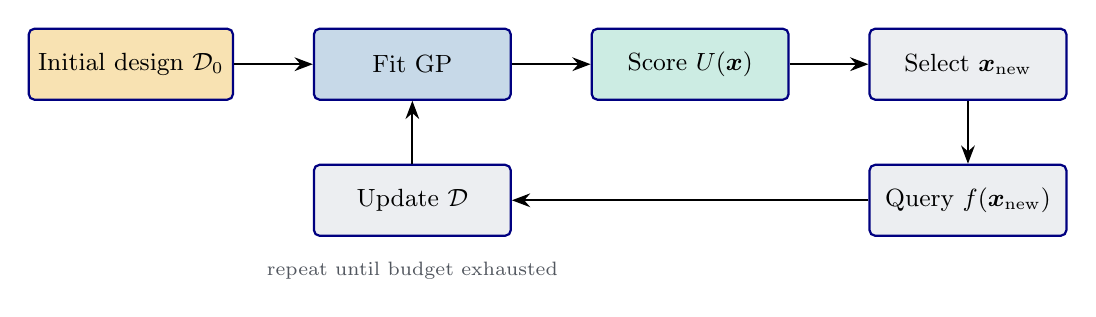
\begin{tikzpicture}[
    mlstep/.style={rectangle, draw=uzhblue, fill=uzhgreylight,
        minimum width=2.5cm, minimum height=0.9cm, font=\small,
        rounded corners=2pt, thick},
    >=Stealth
]
\node[mlstep, fill=softorange!30] (init) {Initial design $\mathcal{D}_0$};
\node[mlstep, right=1cm of init, fill=softblue!30] (gp) {Fit GP};
\node[mlstep, right=1cm of gp, fill=softgreen!20] (score) {Score $U(\x)$};
\node[mlstep, right=1cm of score] (select) {Select $\x_{\text{new}}$};
\node[mlstep, below=0.8cm of select] (query) {Query $f(\x_{\text{new}})$};
\node[mlstep, below=0.8cm of gp] (update) {Update $\mathcal{D}$};

\draw[->, thick] (init) -- (gp);
\draw[->, thick] (gp) -- (score);
\draw[->, thick] (score) -- (select);
\draw[->, thick] (select) -- (query);
\draw[->, thick] (query) -- (update);
\draw[->, thick] (update) -- (gp);

\node[below=0.2cm of update, font=\scriptsize, text=uzhgreydark] {repeat until budget exhausted};
\end{tikzpicture}
\end{center}

\vspace{0.3cm}
\begin{block}{Why this combination works}
\begin{itemize}
  \item \textbf{GP provides UQ:} posterior variance tells us where the approximation is uncertain.
  \item \textbf{BAL selects training points:} maximize information gain per model evaluation.
  \item \textbf{Surrogate = trained GP:} the same GP used for selection serves as the surrogate.
\end{itemize}
\end{block}

{\small Ideal for $d \leq 10$ when each model evaluation costs minutes to hours.}
\end{frame}

% --- Slide 40: Summary Part III ---
\begin{frame}{Summary: Bayesian Active Learning}
\begin{enumerate}
  \item \textbf{BAL} = principled data selection using GP uncertainty.
  \item \textbf{Score function} balances exploration (high $\sigma^2$) and exploitation (high $\mu$).
  \item \textbf{Faster convergence} than uniform sampling, especially for functions with kinks or local features.
  \item \textbf{Application:} surrogate construction for moderate-dimensional problems.
\end{enumerate}

\vspace{0.3cm}
\begin{block}{Hands-on}
\textbf{Notebook:} \texttt{02\_GP\_and\_BAL.ipynb} --- GP from scratch, scikit-learn GP, and BAL comparison.
\end{block}
\end{frame}

% ============================================================================
% PART IV: GAUSSIAN PROCESSES FOR DYNAMIC PROGRAMMING
% ============================================================================

\end{document}
